% This file was created (at least in part) by the script ParseMdtoLatex by Louis du Plessis
% (Available from https://github.com/taming-the-beast)

\documentclass[11pt]{article}
%%%%%%%%%%%%%%%%%%%%%%%%%%%%%%%%%%%%%%%%%%%%%%%%%%%%%%%%%%%%%%%
% DO NOT EDIT THIS FILE UNLESS YOU KNOW WHAT YOU ARE DOING!!! %
%%%%%%%%%%%%%%%%%%%%%%%%%%%%%%%%%%%%%%%%%%%%%%%%%%%%%%%%%%%%%%%

% Useful packages
\usepackage[]{authblk}
\usepackage{graphicx}
\usepackage{color}
\usepackage{longtable}
\usepackage{hanging}
\usepackage{indentfirst}
\usepackage{setspace}
\usepackage{enumitem}
\usepackage{verbatim}
\usepackage{upgreek}
\usepackage{framed}
\usepackage{textcomp}
\usepackage{url}
\usepackage{soul}
\usepackage{amsmath,amsfonts,amssymb,mathrsfs}
\usepackage{fancyhdr}
\usepackage[compact]{titlesec}
\usepackage[T1]{fontenc}
\usepackage{lmodern}
\usepackage[utf8]{inputenc}
\usepackage[]{listings}
%\usepackage{fontspec}
\usepackage{placeins}
\usepackage{epstopdf}
\usepackage[export]{adjustbox}
\usepackage{tikz}
\usepackage[breaklinks]{hyperref}
\usepackage[all]{hypcap}


% References
\usepackage[backend=bibtex,hyperref=true,citestyle=authoryear,bibstyle=authortitle,firstinits=true,terseinits=true,doi=false,url=false,eprint=false,maxbibnames=10,maxcitenames=2]{biblatex}
\DeclareCiteCommand{\cite}
  {\usebibmacro{prenote}}
  {\usebibmacro{citeindex}%
   \printtext[bibhyperref]{\usebibmacro{cite}}}
  {\multicitedelim}
  {\usebibmacro{postnote}}

\DeclareCiteCommand*{\cite}
  {\usebibmacro{prenote}}
  {\usebibmacro{citeindex}%
   \printtext[bibhyperref]{\usebibmacro{citeyear}}}
  {\multicitedelim}
  {\usebibmacro{postnote}}

\DeclareCiteCommand{\parencite}[\mkbibparens]
  {\usebibmacro{prenote}}
  {\usebibmacro{citeindex}%
    \printtext[bibhyperref]{\usebibmacro{cite}}}
  {\multicitedelim}
  {\usebibmacro{postnote}}

\DeclareCiteCommand*{\parencite}[\mkbibparens]
  {\usebibmacro{prenote}}
  {\usebibmacro{citeindex}%
    \printtext[bibhyperref]{\usebibmacro{citeyear}}}
  {\multicitedelim}
  {\usebibmacro{postnote}}

\DeclareCiteCommand{\footcite}[\mkbibfootnote]
  {\usebibmacro{prenote}}
  {\usebibmacro{citeindex}%
  \printtext[bibhyperref]{ \usebibmacro{cite}}}
  {\multicitedelim}
  {\usebibmacro{postnote}}

\DeclareCiteCommand{\footcitetext}[\mkbibfootnotetext]
  {\usebibmacro{prenote}}
  {\usebibmacro{citeindex}%
   \printtext[bibhyperref]{\usebibmacro{cite}}}
  {\multicitedelim}
  {\usebibmacro{postnote}}

\DeclareCiteCommand{\textcite}
  {\boolfalse{cbx:parens}}
  {\usebibmacro{citeindex}%
   \printtext[bibhyperref]{\usebibmacro{textcite}}}
  {\ifbool{cbx:parens}
     {\bibcloseparen\global\boolfalse{cbx:parens}}
     {}%
   \multicitedelim}
  {\usebibmacro{textcite:postnote}}

\newcommand{\citep}{\parencite}
\newcommand{\citet}{\textcite}
\defbibheading{relevref}[\refname]{\section*{Relevant References}}

\renewcommand{\postnotedelim}{\iffieldpages{postnote}{\addcolon}{\addcomma\space}} 
\DeclareFieldFormat{postnote}{#1} 

\DeclareFieldFormat[article, inbook, incollection, inproceedings, patent, thesis, unpublished]{title}{#1}
\DeclareFieldFormat[article, inbook, incollection, inproceedings, patent, thesis, unpublished]{journaltitle}{\mkbibemph{#1}\nopunct}
\DeclareFieldFormat[article, inbook, incollection, inproceedings, patent, thesis, unpublished]{volume}{{#1}\addcolon} %puts volume number in parens
%\DeclareFieldFormat[article, inbook, incollection, inproceedings, patent, thesis, unpublished]{year}{\mkbibparens{#1}\nopunct} %puts year in parens

\DeclareFieldFormat[article, incollection, patent, thesis, unpublished]{pages}{{\nopp#1}}

\DeclareFieldFormat{sentencecase}{\MakeSentenceCase{#1}}

\renewbibmacro*{title}{%
  \ifthenelse{\iffieldundef{title}\AND\iffieldundef{subtitle}}
    {}
    {\ifthenelse{\ifentrytype{article}\OR\ifentrytype{inbook}%
      \OR\ifentrytype{incollection}\OR\ifentrytype{inproceedings}%
      \OR\ifentrytype{inreference}}
      {\printtext[title]{%
        \printfield[sentencecase]{title}%
        \setunit{\subtitlepunct}%
        \printfield[sentencecase]{subtitle}}}%
      {\printtext[title]{%
        \printfield[titlecase]{title}%
        \setunit{\subtitlepunct}%
        \printfield[titlecase]{subtitle}}}%
     \newunit}%
  \printfield{titleaddon}}

\DefineBibliographyStrings{english}{% various adjustments to common bib entry strings
urlseen = {Accessed:},% What goes in front of the date a URL was accessed/retrieved etc.
editor = {(Ed)},%Ed – no dot, in brackets
editors = {(Eds)},% Eds – no dot, in brackets
byeditor = {(Ed.)}}% ‘Edited by’ for edited works

\DeclareNameAlias{default}{last-first}

\renewbibmacro{in:}{}

\renewbibmacro{publisher+location+date}{
  \iflistundef{publisher}
    {}
    {\printlist{publisher}%
       {\addcomma\space}%
      \iflistundef{location}
        {}
        {\printlist{location}}%
    }
}

\DeclareBibliographyDriver{article}{%
\usebibmacro{bibindex}%
\usebibmacro{begentry}%
\usebibmacro{author/translator+others}%
\newunit\newblock
\printfield{year}%
\setunit{\labelnamepunct}\newblock
\usebibmacro{title}%
\newunit
\printlist{language}%
\newunit\newblock
\usebibmacro{byauthor}%
\newunit\newblock
\usebibmacro{bytranslator+others}%
\newunit\newblock
\printfield{version}%
\newunit\newblock
%\usebibmacro{in:}% %mit in:
\usebibmacro{journal}%
\newunit\newblock
\printfield{volume}%
\newunit\newblock
\usebibmacro{byeditor+others}%
\newunit\newblock
\usebibmacro{note+pages}%
\newunit\newblock
\iftoggle{bbx:isbn}
{}%
\newunit\newblock
\usebibmacro{doi+eprint+url}%
\newunit\newblock
\usebibmacro{addendum+pubstate}%
\newunit\newblock
\usebibmacro{pageref}%
\usebibmacro{finentry}}

\DeclareBibliographyDriver{inproceedings}{%
\usebibmacro{bibindex}%
\usebibmacro{begentry}%
\usebibmacro{author/translator+others}%
\newunit\newblock
\printfield{year}%
\setunit{\labelnamepunct}\newblock
\usebibmacro{title}%
\newunit
\printlist{language}%
\newunit\newblock
\usebibmacro{byauthor}%
\newunit\newblock
\usebibmacro{bytranslator+others}%
\newunit\newblock
\printfield{version}%
\newunit\newblock
%\usebibmacro{in:}% %mit in:
\usebibmacro{booktitle}%
\newunit\newblock
\printfield{volume}%
\newunit\newblock
\usebibmacro{byeditor+others}%
\newunit\newblock
\usebibmacro{publisher+location+date}%
\newunit\newblock
\usebibmacro{note+pages}%
\newunit\newblock
\usebibmacro{pageref}%
\usebibmacro{finentry}}

\DeclareBibliographyDriver{book}{%
\usebibmacro{bibindex}%
\usebibmacro{begentry}%
\usebibmacro{author/translator+others}%
\newunit\newblock
\printfield{year}%
\setunit{\labelnamepunct}\newblock
\usebibmacro{title}%
\newunit
\printlist{language}%
\newunit\newblock
\usebibmacro{byauthor}%
\newunit\newblock
\usebibmacro{bytranslator+others}%
\newunit\newblock
%\usebibmacro{in:}% %mit in:
\usebibmacro{booktitle}%
\newunit\newblock
\printfield{volume}%
\newunit\newblock
\usebibmacro{publisher+location+date}%
\newunit\newblock
\usebibmacro{note+pages}%
\newunit\newblock
\usebibmacro{pageref}%
\usebibmacro{finentry}}




% Page margins
\setlength{\evensidemargin}{0in}
\setlength{\headheight}{0in}
\setlength{\headsep}{0in}
\setlength{\oddsidemargin}{-0.25in}
\setlength{\paperheight}{11in}
\setlength{\paperwidth}{8.5in}
\setlength{\tabcolsep}{0in}
\setlength{\textheight}{9in}
\setlength{\textwidth}{7in}
\setlength{\topmargin}{0in}
\setlength{\topskip}{0in}
\setlength{\voffset}{0in}
\parskip = 0.15in
\pagestyle{plain}
\setlength{\parindent}{0cm}

% No white space between list items
\setlist{nolistsep}

% Hyperlink setup
\hypersetup{colorlinks=true,linkcolor=linkscol,citecolor=citescol,urlcolor=urlscol}

% Settings for code blocks
\lstset{backgroundcolor=\color[rgb]{0.972,0.972,0.972},
    tabsize=4,
    rulecolor=,
        basicstyle=\scriptsize,
        upquote=true,
        aboveskip={1.5\baselineskip},
        columns=fixed,
        showstringspaces=false,
        extendedchars=true,
        breaklines=true,
        prebreak = \raisebox{0ex}[0ex][0ex]{\ensuremath{\hookleftarrow}},
        frame=single,
        showtabs=false,
        showspaces=false,
        showstringspaces=false,
        identifierstyle=\ttfamily,
        keywordstyle=\color[rgb]{0,0,1},
        commentstyle=\color[rgb]{0.133,0.545,0.133},
        stringstyle=\color[rgb]{0.627,0.126,0.941}
}

% Colour definitions
\definecolor{citescol}{RGB}{194,101,1}
\definecolor{urlscol}{RGB}{0,150,206}
\definecolor{linkscol}{RGB}{149,0,207}
\definecolor{mycol}{RGB}{25,23,191}
\definecolor{outputcol}{RGB}{34,139,34}
\definecolor{tcol}{RGB}{165,0,14}







% TODO: The rest of the file needs to be cleaned up!
%       Past this point I am not sure what is necessary or not - Louis


\DeclareMathAlphabet{\msfsl}{T1}{cmr}{m}{it}
\DeclareMathAlphabet{\msyf}{OMX}{pcr}{m}{it}
\newcommand{\alf}{\upalpha}
\newcommand{\hilight}[1]{\colorbox{yellow}{#1}}

\newcommand{\levelone}[1]{
\bigskip
\noindent{\LARGE{\textsc{#1}}}
\vspace {0.05in}
}

\newcommand{\leveltwo}[1]{
\bigskip
\noindent{\Large{\textit{#1}}}
\vspace {-1mm}
}

\newcommand{\descriptionhead}[1]{
\noindent{\textcolor{mycol}{\textbf{\textit{#1}}}}\\ \vspace{-7mm}
}

\newcommand{\dhead}[1]{
\noindent{\textbf{\textit{#1 --}}}
}

\newcommand{\exs}[1]{
\vspace{-4mm}
\begin{itemize}
\item #1 \\ \vspace{-8mm}
\end{itemize}
}


\newcommand{\nbo}[1]{{\color{red}{#1}}}


\newcommand{\stepbullet}{\noindent \textbullet \ }
\newcommand{\mi}[1]{\textbf{\textit{#1}}}


\newcommand{\levelthree}[1]{\textit{#1 --}}


%\bibliographystyle{apalike}
%\bibpunct[; ]{(}{)}{;}{a}{,}{;}


\usepackage[breaklinks]{hyperref}
\usepackage[all]{hypcap}
\hypersetup{colorlinks=true,linkcolor=linkscol,citecolor=citescol,urlcolor=urlscol}

% Some macros for software packages
\newcommand{\R}{\texttt{R} }
\newcommand{\TESS}{\texttt{TESS}}
\newcommand{\PBD}{\texttt{PBD}}
\newcommand{\DDD}{\texttt{DDD}}
\newcommand{\Laser}{\texttt{laser}}
\newcommand{\TreePar}{\texttt{TreePar}}
\newcommand{\diversitree}{\texttt{diversitree}}
\newcommand{\RevBayes}{\texttt{RevBayes}}
\newcommand{\Rev}{\texttt{Rev}}
\newcommand{\MrBayes}{\texttt{MrBayes}}
\newcommand{\BEAST}{\texttt{BEAST}}
\newcommand{\PhyloBayes}{\texttt{PhyloBayes}}
\newcommand{\PAML}{\texttt{PAML}}

\let\otheriint\iint
\let\iint\relax
\usepackage{ wasysym }







\definecolor{shadecolor}{RGB}{194,225,255}

\setlength{\tabcolsep}{5pt}
\setlength{\topmargin}{-0.4in}
\setlength{\headheight}{14.5pt}
\pagestyle{fancy}

\newcommand{\taha}[1]{{\textcolor{red}{[TAH comment: #1]}}} % TAH comment

\titlespacing{\section}{0pt}{*0}{*0}
\titlespacing{\subsection}{0pt}{*0}{*0}
\titlespacing{\subsubsection}{0pt}{*0}{*0}

\titleformat{\section}
  {\normalfont\Large\bfseries\color{mycol}}
  {\thesection}{1em}{}

\titleformat{\subsection}
  {\normalfont\large\bfseries\color{mycol}}
  {\thesubsection}{1em}{}

\titleformat{\subsubsection}
  {\normalfont\bfseries\color{mycol}}
  {\thesubsubsection}{1em}{}

% command for MrBayes command-line step
\newcommand{\cl}[1]{{\texttt{\textbf{#1}}}}
\newcommand{\colx}[1]{{\textcolor{tcol}{#1}}}
\newcommand{\mbcl}[1]{\exs{\cl{MrBayes > {#1}}}}

\newcommand{\rbprmt}{RevBayes > } 
\newcommand{\rbcl}[1]{\exs{\cl{\rbprmt{#1}}}}
\newcommand{\rbout}[1]{\exs{\cl{\textcolor{outputcol}{#1}}}}
\newcommand{\rbdn}{{\Large \symbol{126}}} % This makes a copy/pasteable tilde
\newcommand{\rbclml}[1]{\exs{\cl{\ \ \ \ \ \ \ \ \ \ \ {#1}}}}

% text box settings
% requires compiling w/ XeLaTeX
%\newfontfamily\listingsfont[Scale=1.0]{Courier New}
%\lstset{basicstyle=\listingsfont, columns=texcl}
%\defaultfontfeatures{Mapping=tex-text}


\makeatletter
\lst@CCPutMacro\lst@ProcessOther {"2D}{\lst@ttfamily{-{}}{-{}}}
\@empty\z@\@empty
\makeatother



\setlength{\topmargin}{-0.4in}
\setlength{\headheight}{14.5pt}
\pagestyle{fancy}



\definecolor{lg}{gray}{0.75}
\def\gcirc{{%
    \setbox0\hbox{$\fullmoon$}%
    \rlap{\hbox to \wd0{\hss{$\textcolor{lg}{\newmoon}$}\hss}}\box0
}}



% Add your bibtex library here
\addbibresource{master-refs.bib}


%%%%%%%%%%%%%%%%%%%%
% Do NOT edit this %
%%%%%%%%%%%%%%%%%%%%
\begin{document}
\renewcommand{\headrulewidth}{0.5pt}
\headsep = 20pt
\lhead{ }
\rhead{\textsc {Model adequacy using BEAST}}
\thispagestyle{plain}


%%%%%%%%%%%%%%%%%%
% Tutorial title %
%%%%%%%%%%%%%%%%%%
\begin{center}

	% Enter the name of your tutorial here
	\textbf{\LARGE Model adequacy using BEAST v2.4.2}\\\vspace{2mm}

	% Enter a short description of your tutorial here
	\textbf{\textcolor{mycol}{\Large Assessing clock and substitution models}}\\

	\vspace{4mm}

	% Enter the names of all the authors here
	{\Large {\em David A. Duchene}}
\end{center}


%%%%%%%%%%%%%%%%%
% Tutorial body %
%%%%%%%%%%%%%%%%%

\section{Background}\label{background}

This tutorial will guide you through methods to assess model adequacy in BEAST v2.4.2. It is common practice to select evolutionary models based on their statistical fit relative to each other. This might be sufficient in some cases, but there is a risk that all of the candidate models lead to inferences that poorly represent the true evolutionary process. Indeed, even the most complex or best fitting model from a set of candidates can produce highly erroneous estimates of parameters of interest. In this tutorial we will explore methods to investigate the absolute merits of the model. This kind of assessment of the absolute performance of models is also known as model checking or assessment of model adequacy or plausibility.

Before starting the tutorial, it is important that you understand the methods used in Bayesian inference for assessing model adequacy. A typical assessment of model adequacy is done by comparing a test statistic, calculated from the empirical data set, with the values of the statistic calculated from a large number of data sets simulated under the model. The test statistic should be informative about the assumptions of the model in question. The simulated data from the model are frequently referred to as posterior predictive (pps) simulations, and they can be considered as future or alternative data sets under the candidate model. 

Several test statistics have been proposed to assess several of the components of phylogenetic analysis. In this tutorial we will investigate two test statistics, one for assessing the substitution model, and one for assessing the priors on rates and times used for molecular dating (Figure 1). The first statistic is called the multinomial likelihood, which is the likelihood of the data under a model with only a single general assumption: that substitution events are independent and identically distributed. This statistic can be used to assess overall substitution model fit. Note that sites with missing data or indels should not be included when estimating the multinomial likelihood. The second statistic is the \emph{A} index, and assesses the power of the molecular dating model to estimate the number of substitutions across branches, assuming an adequate substitution model is used. We will go through this statistic in more detail during the tutorial.

\begin{figure}
    \centering
    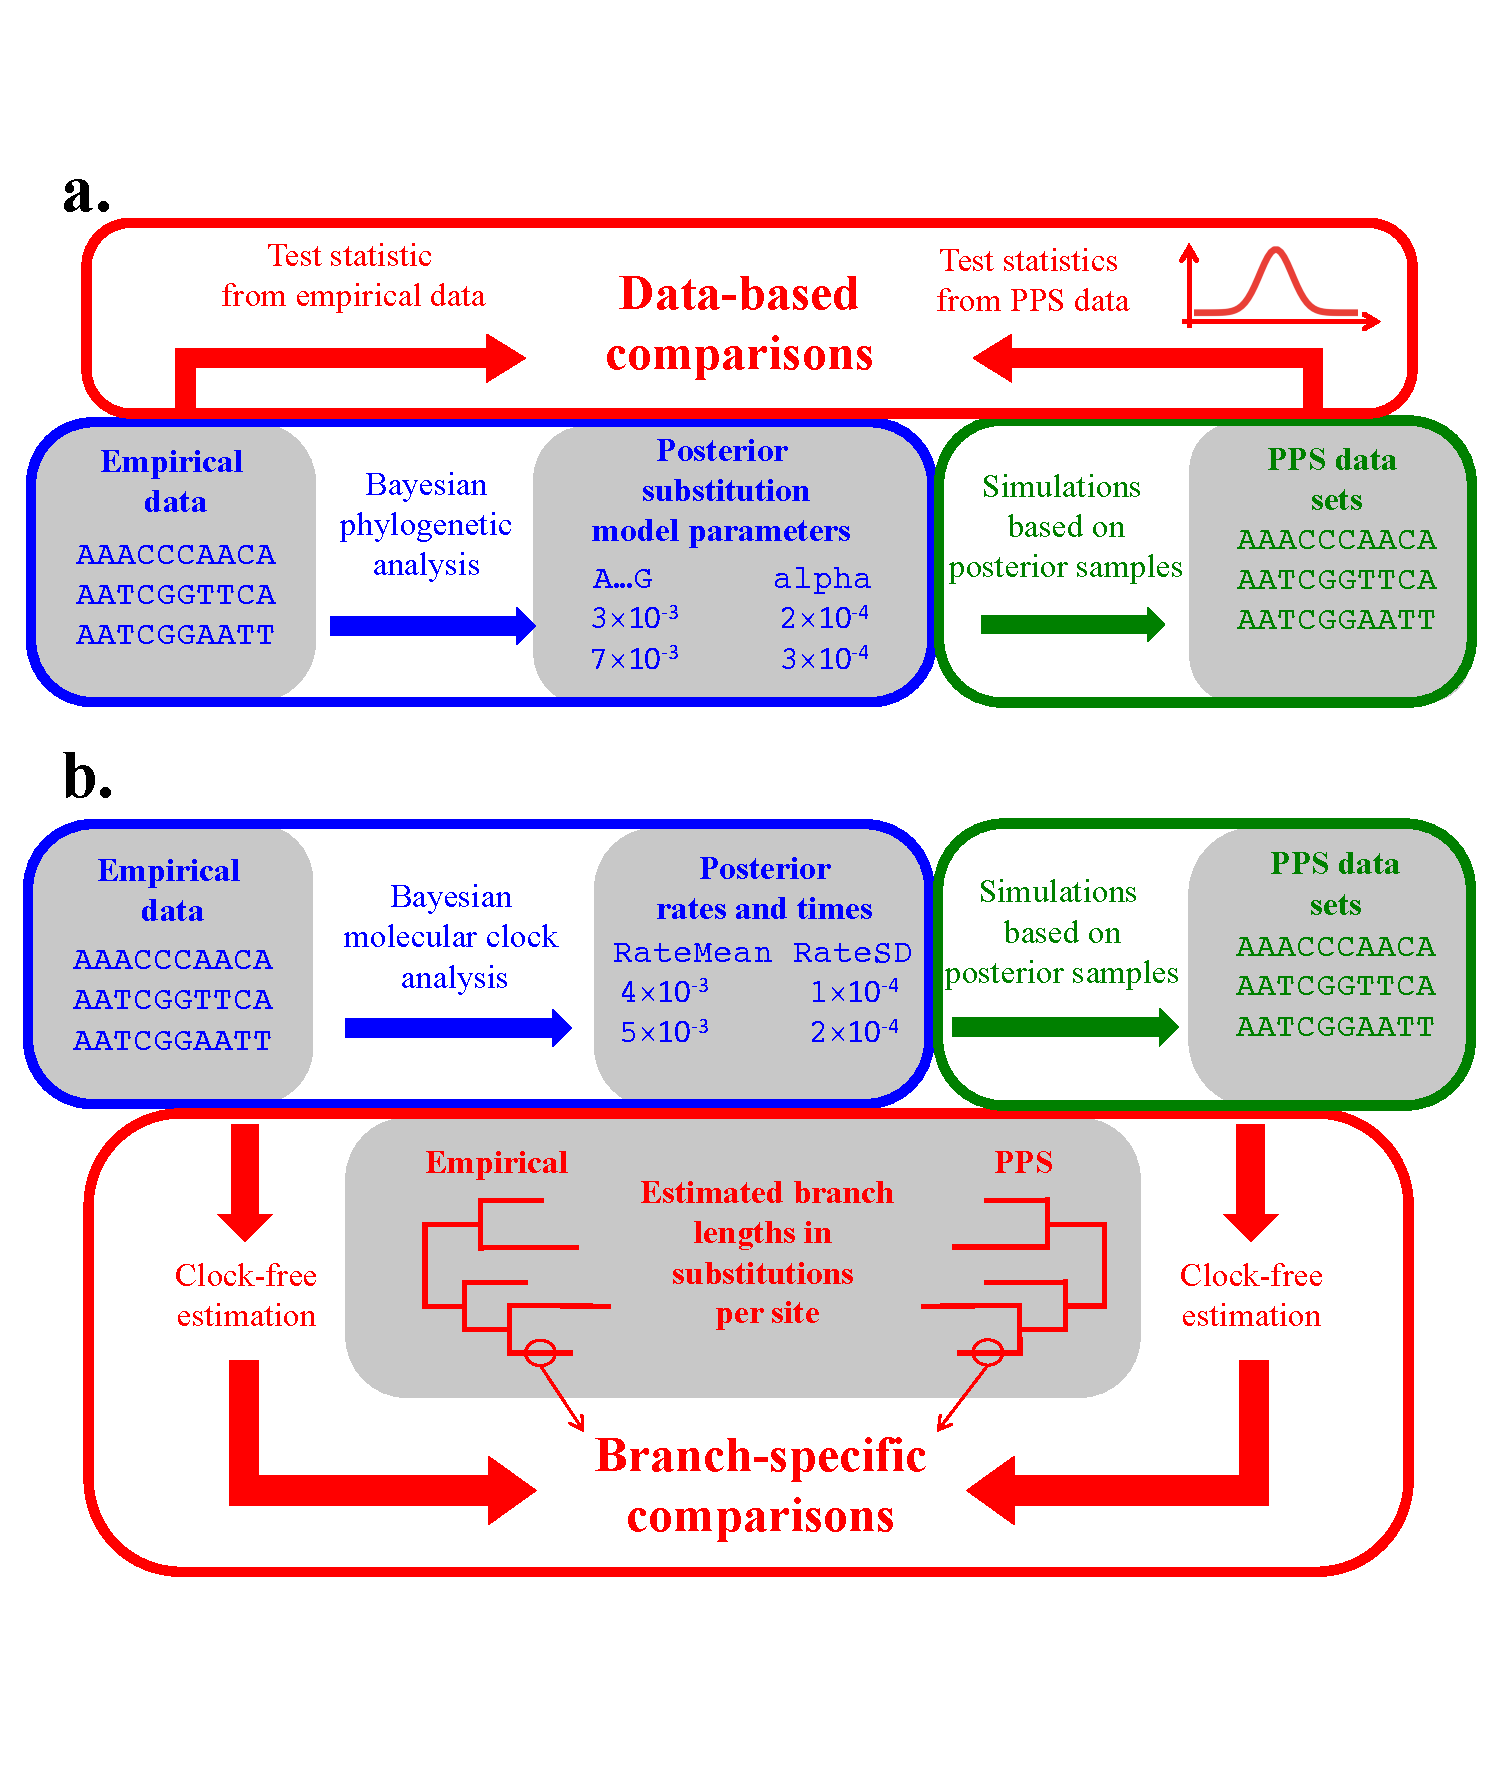
\includegraphics[width=0.800000\textwidth]{figures/Figure_1.pdf}
    \caption{Two of the existing approaches to using posterior predictive simulations to assess model adequacy in Bayesian phylogenetics. (a) One group of methods use characteristics of the data for model assessment, like the multinomial likelihood or the GC content. (b) One method exists that can assess clock models using estimates from clock-free methods. The number of substitutions per site expected along each branch under the clock hierarchical model are then compared with those inferred in a clock-free analysis.}
    \label{fig:example1}
\end{figure}

Please also add a section after the
exercise interpreting the results. End your tutorial with some useful
links.

\section{Programs used in this
Exercise}\label{programs-used-in-this-exercise}

\begin{itemize}

\item
  BEAST2.
\item
  R programming environment.

  \begin{itemize}
  
  \item
     R packages \emph{ape} and \emph{phangorn}.
  \end{itemize}
\end{itemize}

\clearpage

\section{Practical: Steps for assessing model adequacy}\label{practical-Steps-for-assessing-model-adequacy}

\subsection{Step 1: run the empirical data}\label{step-1-run-the-empirical-data}

In the data folder you will find a simulated sequence alignment with 2000 nucleotides in nexus format (al.nex) and a chronogram in newick format (chrono.tre) with 50 taxa. The alignment was simulated along the chronogram under a Jukes-Cantor substitution model and with rate auto-correlation among lineages. You will also find an XML file (sim.xml) in the xml folder to run BEAST 2  for this data set under a strict clock and a Jukes-Cantor model of substitution and a root calibration.

In this first step, we will run the XML file using BEAST 2. The output of this run can also be found in the folder preekooked runs.

\subsection{Step 2: reading the runs and simulating data}\label{step-2-reading-the-runs-and-simulating-data}

To cement the next steps for assessing model adequacy, we will use some of the code in R that we have provided. Specifically, we will explore in detail the file adeq.R. We will first study  the code in R (or the comments) in detail before running the analysis.

The following is the full adeq.R file.

\begin{lstlisting}[language=R]
  adeq <- function(trees.file, log.file, empdat.file, Nsim = 100){
     empdat <- as.phyDat(as.DNAbin(read.nexus.data(empdat.file)))
     seqlen <- ncol(as.matrix(as.DNAbin(empdat)))
     tree.topo <- read.nexus(trees.file)[[1]]
     sims <- make.pps.als(trees.file, log.file, Nsim, seqlen)
     sims <- make.pps.tr(sims, empdat, tree.topo)
     bls <- compile.results(sims)
     return(bls)
 }
\end{lstlisting}

One way to simulate data sets from the model is to use the R package \emph{phangorn}. We first need to read the posterior trees and parameter estimates of your analysis in R. We do this using the function make.pps.als, which identifies the model being assessed and simulates data accordingly. The input for this section includes:

\begin{enumerate}
\def\labelenumi{\arabic{enumi}.}
\item
  The paths of the posterior files for your analysis.
\item
  The number of simulations you want to perform.
\item
  The sequence length (number of sites in your alignment).
\end{enumerate}

 \begin{lstlisting}[language=R]
    sims <- make.pps.als(trees.file, log.file, Nsim, seqlen)
\end{lstlisting}

If the input file has a greater number of samples than the number of simulations requested, this will randomly select samples from the posterior. It is useful at this stage if you make sure you understand how an alignment can be simulated using data from the posterior.

\subsubsection{Step 3: calculate test statistics}\label{step-3-calculate-test-statistics}

Once we have simulated data sets, we can calculate the test statistics. The function make.pps.trs takes the assumed tree, the substitution model, and the empirical and simulated data sets. The function estimates phylogenetic branch lengths for the empirical data set and each of the simulated data sets. In this step we also estimate the multinomial likelihood test statistic for the empirical data and each of the simulated data sets.

 \begin{lstlisting}[language=R]
    sims <- make.pps.tr(sims, empdat, tree.topo)
\end{lstlisting}

The output of this function is what we need for model assessment: the test statistics for the empirical data, and the distribution of values for the simulated data sets.

\subsubsection{Step 4: calculate \emph{P}-values}\label{step-4-calculate-p-values}

We can now compare the test statistic for the empirical data and each of the simulated data sets. The most common way to do this is to calculate the tail area probability, which is the number of simulations with a test statistic greater than the value for empirical data.

 \begin{lstlisting}[language=R]
    bls <- compile.results(sims)
\end{lstlisting}

This function will provide the test statistics for simulations, as well as \emph{P}-values for each of the test statistics. Following practice from frequentist statistics, we can consider the model to be inadequate if the \emph{P}-value for a given test statistic is below 0.05. Importantly, the assessment of the clock model allows us to identify for which branches the molecular dating model can estimate the number of substitutions. We will explore this in the following section.

\subsubsection{Performing model assessment}\label{performing-model-assessment}

The results from the previous steps can be found in the precooked runs folder. The following is example code to run and save the results for clock model adequacy after the BEAST 2 run has completed.

After the BEAST 2 run using the empirical data has completed, the following example code can be run to perform model assessment.

Begin by opening R. The following will set the working directory to the scripts folder, and then source all the functions in the folder.

 \begin{lstlisting}[language=R]
    setwd("[INSERT THE PATH TO SCRIPTS FOLDER]")
    for(i in dir()) source(i)
\end{lstlisting}

Next, we set the directory to precooked runs, and run the function adeq(). The arguments for this function are the posterior of trees in nexus format, the log file, the alignment in nexus format, and the number of posterior predictive simulations to be performed.

\begin{lstlisting}[language=R]
    setwd("../example_run_and_results")
    clock_adequacy_example <- adeq(trees.file = "sim.trees", sim.log ="sim.log", empdat.file = "al.nex", Nsim = 100)
    names(clock_adequacy_example)
\end{lstlisting}

The elements in clock adequacy example are each of the components that can be used to assess clock and substitution model adequacy.

The clock adequacy example object should have the same contents as object "allres" in the file results.Rdata:

\begin{lstlisting}[language=R]
    load("results.Rdata")
    names(allres)
\end{lstlisting}

The following section uses the results from results.Rdata to produce a variety of useful graphics.

\subsubsection{Visualising the results of clock model assessement}\label{visualising-the-results-of-clock-model-assessement}

It is strongly recommended to use qualitative checks of models using graphical analyses. This section uses the results in precooked runs/results.Rdata to graph different components for assessing clock model adequacy using posterior predictive simulations.

The following script shows a simple example to explore the branch wise posterior predictive \emph{P}-values. It requires to have the tree loaded. In this case we will use the original simulated tree, but usually the tree with the median posterior branching times would be appropriate. We will colour the branches with good accuracy in blue, and the branches that have poor accuracy in green (Figure 2).

\begin{lstlisting}[language=R]
   tr <- read.tree("chrono.tre")
   plot(tr, edge.col = rainbow(length(allres$branch_wise_pppvalues), start = 2/6, end = 4/6)[
   		rank(allres$branch_wise_pppvalues)], edge.width = 6, cex = 1.5)
   edgelabels(allres$branch_wise_pppvalues, bg = "white", cex = 1.5, frame = "none")
\end{lstlisting}

\begin{figure}
    \centering
    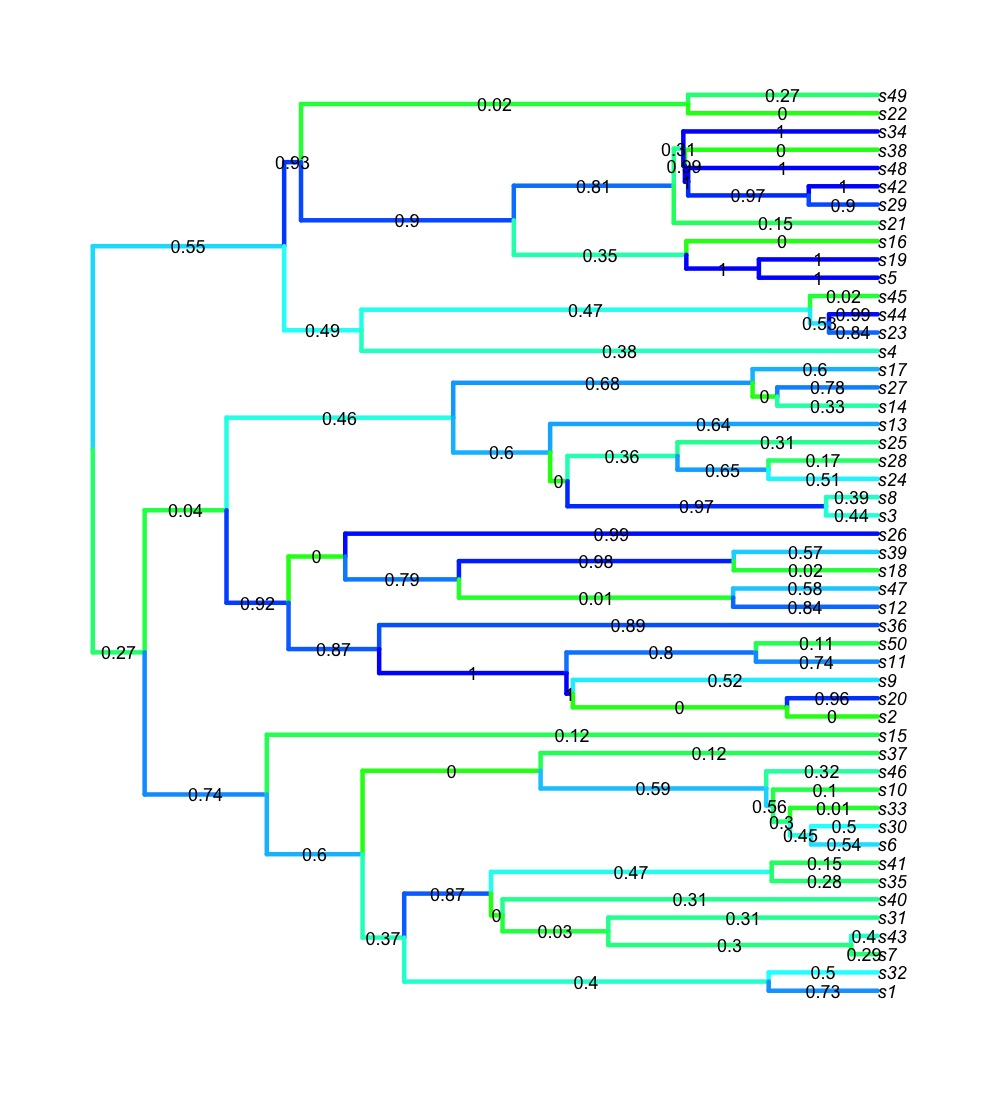
\includegraphics[width=0.800000\textwidth]{figures/Figure_2_branchwise_p.jpg}
    \caption{Estimated chronogram with branches coloured by their clock adequacy \emph{P}-value.}
    \label{fig:example2}
\end{figure}

The following script shows a simple example to explore the branch wise length deviation, which is another metric for accuracy. We apply the same colouring system as the plot above, but note that in the case of branch length deviation larger numbers indicate greater deviation from the empirical branch length, and therefore lower accuracy (Figure 3).

\begin{lstlisting}[language=R]
    plot(tr, edge.col = rainbow(length(allres$branch_length_deviation), start = 4/6, end = 2/6)[rank
    		(allres$branch_length_deviation)], edge.width = 6, cex = 1.5)
    edgelabels(round(allres$branch_length_deviation, 2), bg = "white", cex = 1.5, frame = "none")
\end{lstlisting}

\begin{figure}
    \centering
    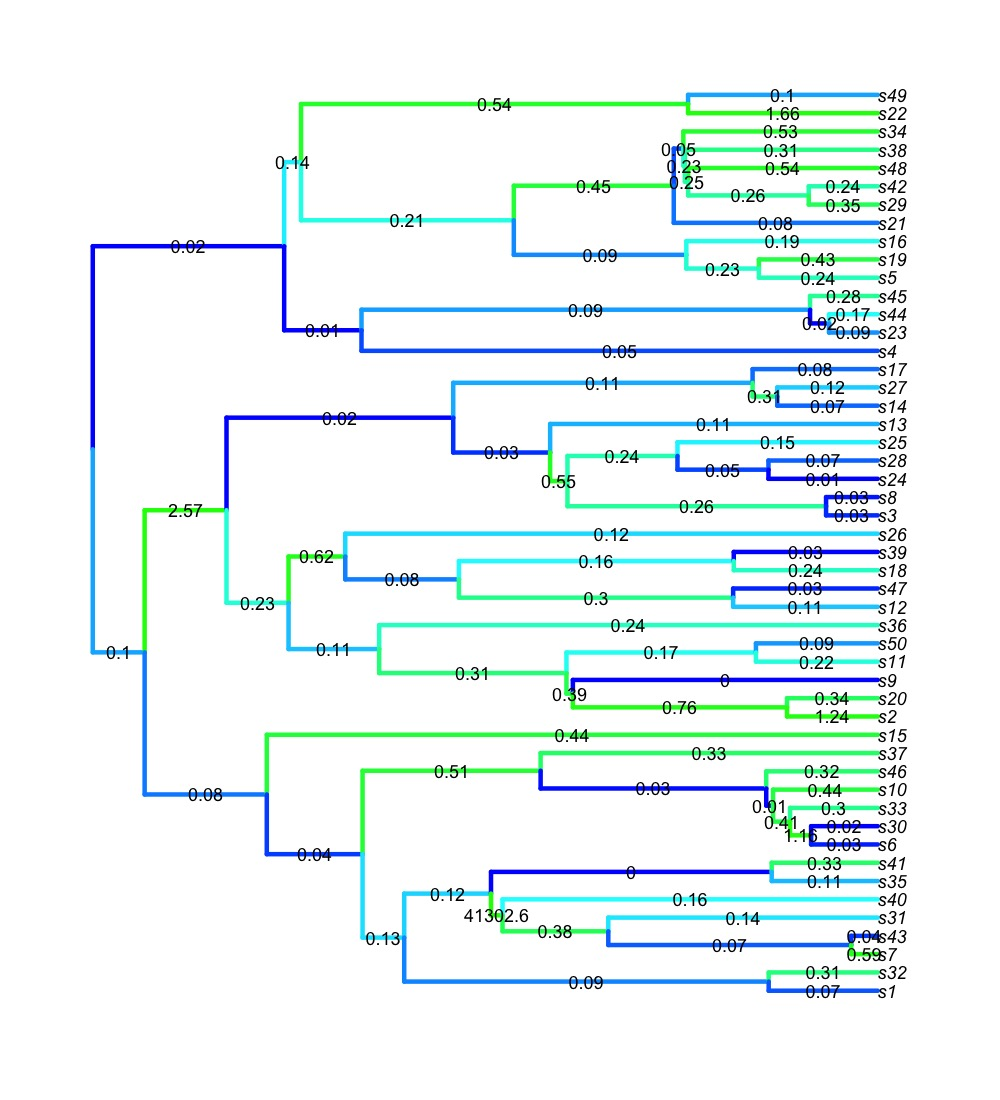
\includegraphics[width=0.800000\textwidth]{figures/Figure_3_branchwise_dev.jpg}
    \caption{Estimated chronogram with branches coloured by their deviation between the empirical and simulated lengths.}
    \label{fig:example3}
\end{figure}

Note that in this simple method to graph the results, the branches in the two plots above have been coloured by their rank, rather than their magnitude.

\section{Useful references}\label{useful-references}

\begin{itemize}

\item
  Goldman, N. (1993). Statistical tests of models of DNA substitution. Journal of molecular evolution, 36(2), 182-198.
\item
  Bollback, J. P. (2002). Bayesian model adequacy and choice in phylogenetics. Molecular Biology and Evolution, 19(7), 1171-1180.
\item
  Duchene, D. A., Duchene, S., Holmes, E. C., & Ho, S. Y. (2015). Evaluating the adequacy of molecular clock models using posterior predictive simulations. Molecular biology and evolution, 32(11), 2986-2995.
\end{itemize}

\clearpage



%%%%%%%%%%%%%%%%%%%%%%%
% Tutorial disclaimer %
%%%%%%%%%%%%%%%%%%%%%%%
% Please do not change the license
% Add the author names and relevant links
% Add any other aknowledgments here
\href{http://creativecommons.org/licenses/by/4.0/}{
\includegraphics[scale=0.8]{figures/ccby.pdf}} This tutorial was written by David A. Duchene for \href{https://taming-the-beast.github.io}{Taming the BEAST} and is licensed under a \href{http://creativecommons.org/licenses/by/4.0/}{Creative Commons Attribution 4.0 International License}. 


%%%%%%%%%%%%%%%%%%%%
% Do NOT edit this %
%%%%%%%%%%%%%%%%%%%%
Version dated: \today



\newpage

%%%%%%%%%%%%%%%%
%  REFERENCES  %
%%%%%%%%%%%%%%%%

\printbibliography[heading=relevref]


\end{document}